\chapter{Experiments}

\section{Experiments on a real-time data stream}

\begin{wrapfigure}{r}{0.4\textwidth}
  \begin{center}
    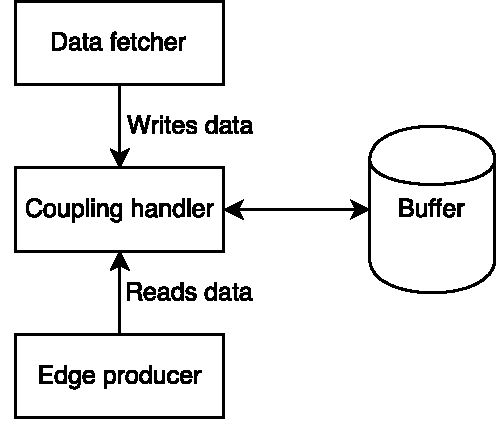
\includegraphics[width=0.38\textwidth]{Pipeline}
  \end{center}
  \caption{Parallel-compatible pipeline layout}
  \label{fig:pipeline}
\end{wrapfigure}

To do real-time experiments on a data stream there are a few more tasks that needs to be performed. The three main tasks are: fetch data, produce graph edges and update DANF. To efficiently perform these tasks they are run in parallel. They are implemented as components of a pipeline as seen in figure \ref{fig:pipeline}. A component stores its results in a buffer which can be read by the component next in the pipeline. The writing component has write-only access and the reading component has read-only access. Note that Edge producer can be a writer to a DANF updater using another coupling handler. This makes it possible to create a theoretically infinite pipeline with very low coupling between components and allows every component to run in their own threads.

As all nodes and edges are handled as plain numbers, a mapping needs to be stored from node index to the data. To avoid the data manager from competing with the algorithm for CPU and memory, the data should preferably be stored in a database by a completely different machine. The only data that needs to be saved on the same machine as the algorithm is a mapping from node index to data index, which can be saved on disk.

A list of the calculated value for each node is kept in a list $A$. Another list $B$ keeps track of the value of the nodes that change. After a given amount of time, the difference of the changed nodes are checked and nodes with significant changes are marked as rapidly changing. The elements in $B$ is added to $A$ and $B$ is cleared. This allows the detection of upcoming trends. 

Another useful feature used was to keep track of the top nodes, sorted in descending order according to their DANF values. Initially, all nodes were tracked. However, this turned out to be unsustainable on a graph with only a few millions of nodes. Instead, only the top most $X$ nodes were tracked. This leads to a drastic speed increase while still being able to check which are the most central nodes. 


\subsection{Graph layout}

When performing experiments on the data-stream a certain graph structure was used. The structure was designed to be able to detect popular subjects, authors and sources. This was achieved by creating three different graph models which, for simplicity, were combined into one, see figure \ref{fig:experiment-graph}. The common node for all models is Document. 

The first model is the concept to document part. This model identifies popular subjects by retrieving all concepts that are mentioned in a document and then adding an edge from the concept to the document. The DANF value represents how many mentions a concept have. 

The second model is the location to document line in the middle. This model can identify which locations, sources (news) and authors that publishes the most documents.

The last model is the named entity part to the right in the figure. The named entities are general things mentioned in articles; such as countries, people or companies. Each entity has a sentiment. The sentiment specifies if the entity is mentioned in a positive (P), neutral (N) or negative (V) manner. Using the visualized structure for the named entities in figure \ref{fig:experiment-graph} enables detection of both the number of mentions and trends of how entities are referenced.

\begin{figure}[h]
\centering
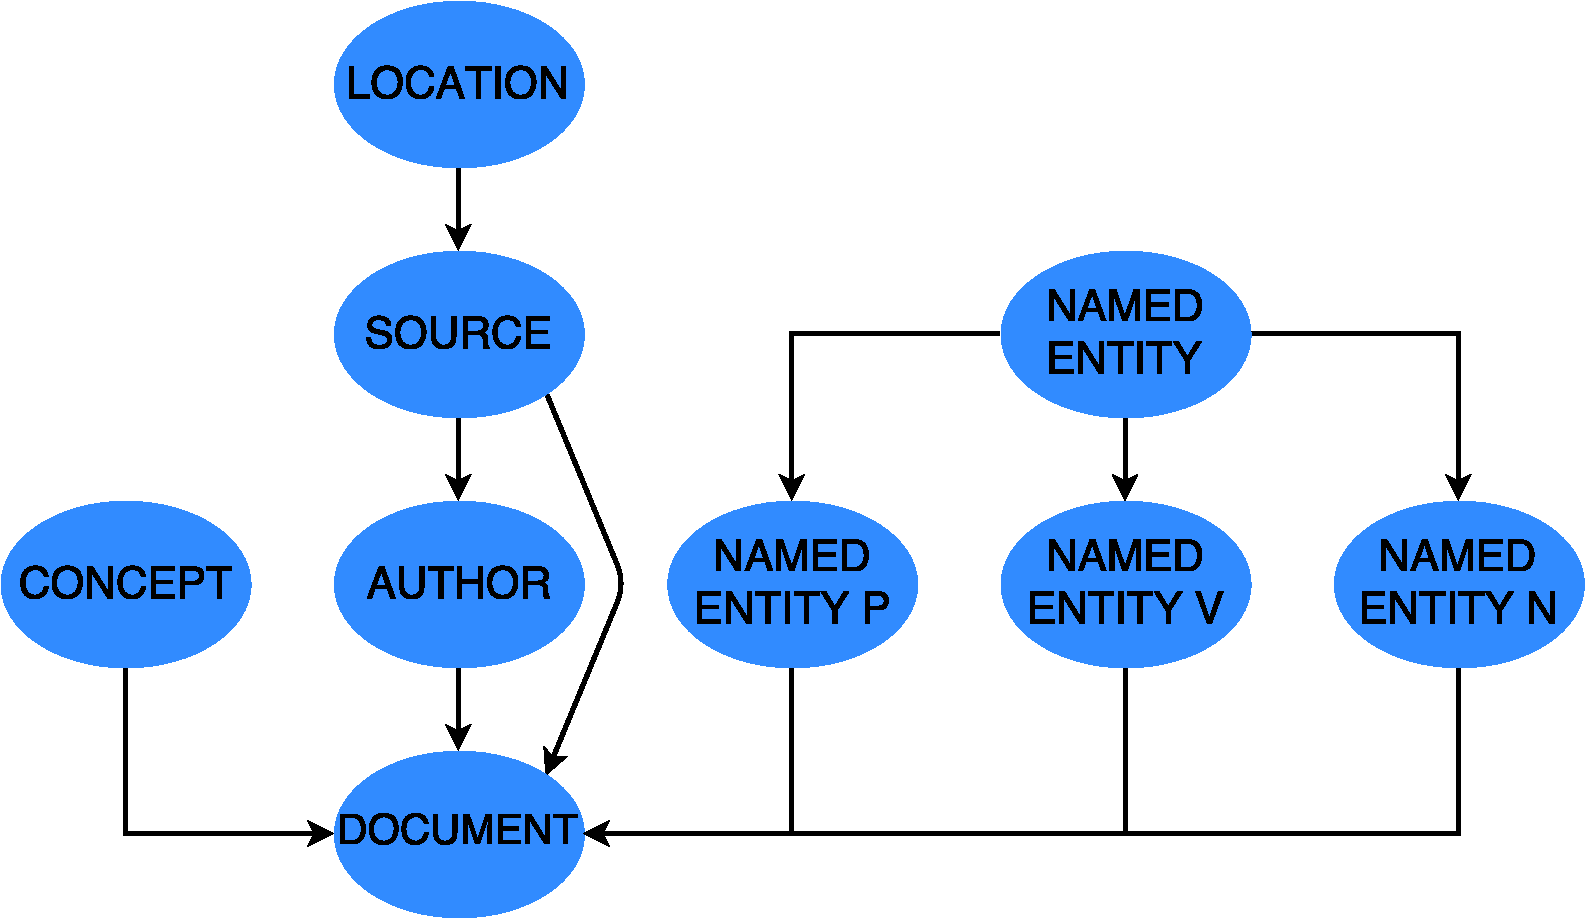
\includegraphics[width=\textwidth]{Graph}    
\captionsetup{justification=centering}
\caption {Graph layout used in the conducted experiment}
\label{fig:experiment-graph}
\end{figure}


\subsection{Starting with an empty graph}

The first experiment performed was done by creating an initially empty graph and setting up DANF to track the neighborhood function on it. A connection was established to the company live stream. The algorithm had no trouble keeping up with the stream of about 11 documents per second (two million documents per day) where about 30 edges were generated per document. 

\subsection{Starting with an arbitrary large graph}

Building a large graph from the existing data would take a long time. The data would have to be parsed and analyzed to generate edges. Instead of spending a large amount of time to generate the graph the it-2004 graph, see Appendix \ref{appendix4}, was used. DANF managed about ten or eleven documents per second, which means that it could not quite keep up with the stream. This indicates that roughly one billion edges are the limit of the current implementation, but the it-2004 graph is more dense than the constructed graph so DANF would have a higher performance if the graph was made from scratch. More optimizations are required to prevent buffer build up in the long run. 

\subsection{Data retrieval}
From the experiment it was evident that both the United States and China were central nodes in the constructed graph. The United States was one of the most central node in all of the three models.

In the experiment, a trend concerning North Korea was detected. Short after North Korea released information concerning further nuclear tests, the DANF value of the North Korean concept node increased rapidly. Such trends can easily be detected by tracking rapidly changing nodes.
